% This is samplepaper.tex, a sample chapter demonstrating the
% LLNCS macro package for Springer Computer Science proceedings;
% Version 2.20 of 2017/10/04
%
\documentclass[runningheads]{llncs}
\usepackage[a4paper, margin=1in]{geometry}
\usepackage{minted}
\usepackage[export]{adjustbox}
\usepackage{wrapfig}
\usepackage{url}
%
\usepackage{graphicx}
\renewcommand\labelitemi{\raisebox{0.4ex}{\tiny$\bullet$}}
\renewcommand{\labelitemii}{$\cdot$}
% Used for displaying a sample figure. If possible, figure files should
% be included in EPS format.
%
% If you use the hyperref package, please uncomment the following line
% to display URLs in blue roman font according to Springer's eBook style:
% \renewcommand\UrlFont{\color{blue}\rmfamily}

\begin{document}
%
\title{Auto-Indexing in PostgreSQL}
%
%\titlerunning{Abbreviated paper title}
% If the paper title is too long for the running head, you can set
% an abbreviated paper title here
%
\author{Vamsi Krishna Reddy Satti \and
Vighnesh Reddy Konda \and
\\Niranjan Vaddi \and
Sai Praneeth Reddy Sunkesula}
%
\authorrunning{Vamsi, Vighnesh, Niranjan, Praneeth}
% First names are abbreviated in the running head.
% If there are more than two authors, 'et al.' is used.
%
\institute{Department of Computer Science and Engineering,\\
Indian Institute of Technology Bombay, Mumbai, India\\
\email{\{160050064, 160050090, 160050099, 160050100\}@iitb.ac.in}}\\
%
\titlerunning{Auto-Indexing in PostgreSQL}
\maketitle              % typeset the header of the contribution
%
\begin{abstract}
Indexing the tables in database systems can increase efficiency based on the types of operations done on the tables. PostgreSQL does not enable indexing on non primary key columns by default. However indexing can be useful when there are frequent reads from similar columns on the table. 
We implemented an application for PostgreSQL to detect the columns that needs to be indexed based on the frequency of scans done by postgreSQL and create indexes for those columns. By this the database adapts and access patterns improve as the workload changes without any human intervention in cases where the reads are more frequent than writes. We implemented this by extracting the queries on the database from a custom logfile.

\end{abstract}
%
%
%


\section{Query Processing in PostgreSQL}
\subsection{Introduction}
The \texttt{exec\_simple\_query} function in \texttt{postgres.c} can be summarized as follows:

\begin{minted}
[
frame=lines,
framesep=2mm,
fontsize=\footnotesize,
linenos
]
{c}
static void
exec_simple_query(const char *query_string)
{
	...
	List *parsetree_list = pg_parse_query(query_string);
	...
	foreach(parsetree_item, parsetree_list)
	{
		List *querytree_list = pg_analyze_and_rewrite(parsetree, query_string, NULL, 0, NULL);
		List *plantree_list = pg_plan_queries(querytree_list, CURSOR_OPT_PARALLEL_OK, NULL);
		...
		PortalDefineQuery(portal, NULL, query_string, commandTag, plantree_list, NULL);
		PortalStart(portal, NULL, 0, InvalidSnapshot);
		...
		(void) PortalRun(portal, FETCH_ALL, isTopLevel, true, receiver, receiver, completionTag);
		PortalDrop(portal, false);
	}
}
\end{minted}

The code snippet above suggests that PostgreSQL processes each SQL command in a four step process:
\begin{enumerate}
\item Parse
\item Analyze and Rewrite
\item Plan
\item Execute
\end{enumerate}

\begin{figure}
    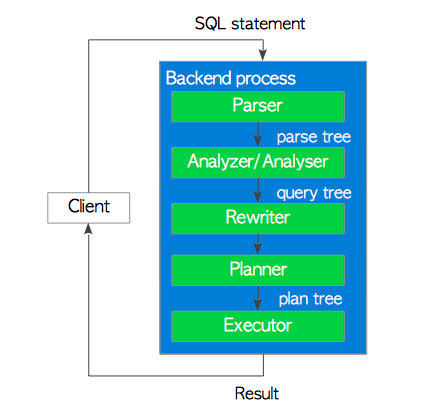
\includegraphics[scale=0.5,center]{images/query_processing.png}
\end{figure}


\subsection{Parse}
Internally PostgreSQL converts the SQL query string to an internal data structure, referred to as parse tree.

Simply speaking, PostgreSQL uses  a parser generator called Bison, in which the grammar rules for query syntax is defined. Bison generates a parser code using the PostgreSQL build process. The generated parser code is what runs inside of Postgres when we send it SQL commands. Each grammar rule is triggered when the generated parser finds a corresponding pattern or syntax in the SQL string, and inserts a new C memory structure into the parse tree data structure.

\subsection{Analyze and Rewrite}
Once PostgreSQL has generated a parse tree, it then converts it into a another tree structure using a different set of nodes. We can see all this work in another C function \texttt{pg\_analyze\_and\_rewrite}.

The analyze and rewrite process applies a series of sophisticated algorithms and heuristics to try to optimize and simplify your SQL statement. If you had executed a complex select statement with sub-selects and multiple inner and outer joins, then there is a lot of room for optimization. It’s quite possible that PostgreSQL could reduce the number of sub-select clauses or joins to produce a simpler query that runs faster.

\subsection{Plan}
The last step Postgres takes before starting to execute our query is to create a plan (a plan tree). This involves generating a tree of nodes that form a list of instructions for PostgreSQL to follow.

The C function that starts the query planning process is called \texttt{pg\_plan\_queries}.

\subsection{Execute}
Now, finally PostgreSQL follows the plan to execute the query. At each type of node that PostgreSQL encounters while traversing the tree, it utilizes the corresponding \texttt{Exec*} function to run the appropriate logic and get the tuples. For this, \texttt{exec\_simple\_query} opens a portal which is an abstraction for executing the plans generated from planner.

\newpage 

\section{Query Logging and Table-Column extraction}
The automatic indexer processes on the select statements on tables present in data schema. So we are logging only select queries into a different file from the ExecutorEnd function of the postgresql executor (\url{src/backend/executor/execMain.c}). Every log line is a tuple of the form (timestamp, query statement, cost as estimated by query planner).  

The backend program then reads this line whenever the log file changes (this is done using linux tail command). The query is fingerprinted to in order to group similar queries. The tables, columns used in that query are then extracted by parsing the query plan. This table-column extraction is done once per a fingerprint in order to avoid extra overhead.

\section{Indexing Strategies Used}
The strategy implemented for automatic indexing is a close variant of the ski-rental strategy. The steps and features involved are :

\begin{enumerate}
    \item When a query is executed, the reduction in cost of execution is estimated by creating hypothetical index using the HypoPG extension (this does not have any overhead as it does not actually create indexes). Various possible index combinations are generated using the result from the query plan parser. The index combinations include
    \begin{itemize}
        \item Basic indexing on one column of a table which was accessed during the execution of query.
        \item Permutations of multi-indexing on two columns of a table
        \item Multi-indexing on a set of columns of a table which occur together in a conjunction, which is a sub part of the query condition
    \end{itemize}
    \item The query chooses the best possible indexing combination from the above,  based on the cost reduction due to indexing.
    \item This cost difference is accumulated to the corresponding fingerprint after reducing the previous aggregate by a decaying exponential function of time. This metric indicates the improvement of query execution for this fingerprint queries, if the indexing were created before executing the queries. The exponential decaying ensures the older queries get lesser priority in indexing. 
    \item Index creation overhead is assumed to be a linear function in the size of rows, since the base of the logarithmic part is very large. The number of rows is being obtained from the database metadata relation \textbf{pg\_class}
    \item Indexing is done on the table if the improvement due to indexing (as computed in step 3) is greater than the index creation overhead. This technique limits the extra cost incurred due to not doing indexing optimally to twice the extra cost incurred by optimal indexing.
    \item The indices which are not used frequently are dropped out, using a seperate thread which drops an index on a table if the frequency estimate falls below a threshold. An exponentially decaying time factor with is used to achieve this. Synchronization between this thread and the main thread is achieved via locks.
    \item \textbf{Optimization} : In order to prevent extra overhead on database due the \textbf{explain} statements executed during hypothetical indexing, the cost before indexing which is obtained along with the query log is used to identify any updates on the tables. So the number of rows estimation and hypothetical indexing will be done only if there are no updates on the tables. However, Query Plan must be acquired once when first query of a fingerprint is executed for table-column extraction (as discussed in previous section). 
\end{enumerate}

\newpage

\section{Utilizing PostgreSQL Internals for efficiency}

Since our code initially depended completely on PostgreSQL logs for determining the strategies to be used and index creation/drop decisions, we tried to optimize this by extracting the required data directly while a query is being executed inside PostgreSQL by modifying its source and recompiling it. 

Instead of calling an explain again for every query run to get the details of estimated cost of execution in PostgreSQL, we directly added the following code snippet before \texttt{ExecutorEnd} starts doing its work (in file \texttt{src/backend/executor/execMain.c}).

\begin{minted}
[
frame=lines,
framesep=2mm,
fontsize=\footnotesize,
linenos
]
{c}
void
ExecutorEnd(QueryDesc *queryDesc) {
        // Added code here -------
	if (queryDesc->operation == CMD_SELECT) {
    	    // fptr is the pointer to our custom log file
		fprintf(fptr, "%lu,\"%s\",%f\n", (unsigned long) time(NULL),
		    queryDesc->sourceText, queryDesc->planstate->plan->total_cost);
		fflush(fptr);
	}
	// ------------------------
	if (ExecutorEnd_hook)
		(*ExecutorEnd_hook) (queryDesc);
	else
		standard_ExecutorEnd(queryDesc);
}
\end{minted}

This code logs the UNIX timestamp, the original query string and the estimated cost present in the plan into our file.

\subsection{Other possible optimizations}

Rather than parsing the query plan using an explain once for every new query (with respect to fingerprint), we could directly get the columns names and corresponding tables inside from, where, having, group by \textit{etc.} clauses using the parse tree from the parser. Though, we could not get the code working for this in due time, a brief overview on how this can be done is as follows.

Firstly, lets look at the  \texttt{Query} structure from \texttt{/src/include/nodes/parsenodes.h} as shown below partially.

\begin{minted}
[
frame=lines,
framesep=2mm,
fontsize=\footnotesize,
linenos
]
{c}

/*
 * Query -
 *	  Parse analysis turns all statements into a Query tree
 *	  for further processing by the rewriter and planner.
 *
 *	  Utility statements (i.e. non-optimizable statements) have the
 *	  utilityStmt field set, and the rest of the Query is mostly dummy.
 *
 *	  Planning converts a Query tree into a Plan tree headed by a PlannedStmt
 *	  node --- the Query structure is not used by the executor.
 */
typedef struct Query
{
	NodeTag		type;
	CmdType		commandType;	/* select|insert|update|delete|utility */
	QuerySource querySource;	/* where did I come from? */
	uint32		queryId;		/* query identifier (can be set by plugins) */
	bool		canSetTag;		/* do I set the command result tag? */
	Node	   *utilityStmt;	/* non-null if commandType == CMD_UTILITY */
    ...
	List	   *cteList;		/* WITH list (of CommonTableExpr's) */
	List	   *rtable;			/* list of range table entries */
	FromExpr   *jointree;		/* table join tree (FROM and WHERE clauses) */
	List	   *targetList;		/* target list (of TargetEntry) */
    ...
	List	   *returningList;	/* return-values list (of TargetEntry) */
	List	   *groupClause;	/* a list of SortGroupClause's */
	List	   *groupingSets;	/* a list of GroupingSet's if present */
	Node	   *havingQual;		/* qualifications applied to groups */
	List	   *windowClause;	/* a list of WindowClause's */
	List	   *distinctClause; /* a list of SortGroupClause's */
	List	   *sortClause;		/* a list of SortGroupClause's */
	Node	   *limitOffset;	/* # of result tuples to skip (int8 expr) */
	Node	   *limitCount;		/* # of result tuples to return (int8 expr) */
    ...
} Query;
\end{minted}

The \texttt{jointree} attribute contains all the tables present in the from clause. The \texttt{targetList} contains the columns we would like every tuple result to be projected into. The \texttt{sortClause} keeps the order by attributes in the original query and similarly for other clauses too. Importantly, the rtable (i.e. the range table entries) contain the aliases the user might have used and quals present inside jointree indicate the where consitions over which the tuples are to be found for.

So, we can see that a lot of this information about the various column accesses and conditions are already present in this structure from the parser. But, unfortunately, we couldn't really utilize this potential in our implementation. We could only get the OIDs (the identities PostgreSQL uses to identify tables and columns) of columns accesses of corresponding tables for query type from a limited set.

\section{External Packages used}

Our experiemnts and results are all based on machines using PostgreSQL 10.5

\subsection{psycopg2}
This is a PostgreSQL client in Python3 for executing SQL queries from external programs in Python. We used this package for our complete interaction with database, including the testing procedure.

\subsection{HypoPG}
[\url{https://github.com/HypoPG/hypopg}] - This package is used for hypothetically indexing a table to estimate the performance gain due to indexing which is required for the solving ski-rental problem. The interesting deal about this is that the indices are not actually created in the database, but just extimates costs in plan as if the given indices were present.

\subsection{libpg\_query}
[\url{https://github.com/lfittl/libpg\_query}] - We use this C library for fingerprinting queries \textit{i.e.} to group up queries that are similar in their parse tree structure by performing a SHA1 hash through the tree.

\begin{minted}
[
frame=lines,
framesep=2mm,
fontsize=\footnotesize,
linenos
]
{c}
void
_fingerprintNode(FingerprintContext *ctx, const void *obj, const void *parent, 
            char *field_name, unsigned int depth) {
    ...
    if (IsA(obj, List)) {
        _fingerprintList(ctx, obj, parent, field_name, depth);
    }
    else {
        switch (nodeTag(obj)) {
            case T_Integer:
                ...
            case T_Float:
                ...
            case T_SelectStmt:
                ...
            // other cases continue
        }
    }
}
\end{minted}

A brief description of its working is as follows. We have the parse tree after \texttt{pg\_parse\_query} in \texttt{src/backend/tcop/postgres.c} executes to give \texttt{parsetree\_list} in \texttt{exec\_simple\ query}. So, we modified the source of PostgreSQL to call our function \texttt{DB\_Project\_GetFingerprint} to log the fingerprint of this query into our custom log file. This function creates a memory context for this task of fingerprinting and calls a recursive function \texttt{\_fingerprintNode} to traaverse the tree. Now if the node is a leaf, \textit{i.e.} not a \texttt{List}, the type of node is checked and correspondingly on a case-by-case basis, fingerprint the node accordingly as shown above.

\begin{minted}
[
frame=lines,
framesep=2mm,
fontsize=\footnotesize,
linenos
]
{c}
static void
_fingerprintSelectStmt(FingerprintContext *ctx, const SelectStmt *node, const void *parent,
                const char *field_name, unsigned int depth)
{
  _fingerprintString(ctx, "SelectStmt");

  if (node->all) {
    _fingerprintString(ctx, "all");
    _fingerprintString(ctx, "true");
  }

  if (node->distinctClause != NULL && node->distinctClause->length > 0) {
    _fingerprintNode(&subCtx, node->distinctClause, node, "distinctClause", depth + 1);
  }
  if (node->fromClause != NULL && node->fromClause->length > 0) {
    _fingerprintNode(&subCtx, node->fromClause, node, "fromClause", depth + 1);
  }
  if (node->groupClause != NULL && node->groupClause->length > 0) {
    _fingerprintNode(&subCtx, node->groupClause, node, "groupClause", depth + 1);
  }
  if (node->havingClause != NULL) {
    _fingerprintNode(&subCtx, node->havingClause, node, "havingClause", depth + 1);
  ...
  // simialr if conditions on all other clauses and quals select statement carries
  ...
  }
\end{minted}

For example, we look at the case when a (leaf) node is tagged as \texttt{T\_SelectStmt} which indicates a select statement as shown above. Now, the fingerprint algorithm runs through any fromClause, groupClause, havingClause \textit{etc.} and hashes their existence accordingly, thus identifying similar queries with same hashes.

\section{Future Scope of Work}


\begin{itemize}
    \item Currently, the query log is redirected to a file from which the external application reads and processes for indexing. Instead we can create a relation in the database to store the log and query the log from the external application. This can reduce disk I/O overheads on the indexing application.
    \item For dropping out unused indexes, we are currently considering only a time factor. By keeping track of the overhead due to the index on updates on the table, it is possible to drop indexes in a similar but reverse method as creating the indices i.e whenever the aggregate overhead scaled by the time factor exceeds a threshold, drop the index.
\end{itemize}


%
% ---- Bibliography ----
%
% BibTeX users should specify bibliography style 'splncs04'.
% References will then be sorted and formatted in the correct style.
%
% \bibliographystyle{splncs04}
% \bibliography{mybibliography}
%
\begin{thebibliography}{8}

\bibitem{ref_interdb}
Hironobu Suzuki: The Internals of PostgreSQL 
\url{http://www.interdb.jp/pg/}

\bibitem{ref_pat_shaughnessy}
Pat Shaughnessy: Following a Select Statement Through Postgres Internals \url{http://patshaughnessy.net/2014/10/13/following-a-select-statement-through-postgres-internals}

\bibitem{ref_postgres_internals}
PostgreSQL Internals Through Pictures \url{https://www.postgresql.org/files/developer/internalpics.pdf}

\bibitem{ref_oracle}
Selecting an Index Strategy \url{https://docs.oracle.com/cd/B12037_01/appdev.101/b10795/adfns_in.htm}

\bibitem{ref_microsoft_azure}
Automatic index management in Azure SQL database
\url{https://blogs.msdn.microsoft.com/sqlserverstorageengine/2017/05/16/automatic-index-management-in-azure-sql-db/}

\bibitem{ref_hypopg}
HypoPG Extension for PostgreSQL
\url{https://github.com/HypoPG/hypopg}

\bibitem{ref_psycopg2}
Psycopg2 - PostgreSQL database connector for Python3 for running PostgreSQL statements from external program.
\url{http://initd.org/psycopg/docs/}

\end{thebibliography}
\end{document}
